\documentclass[11pt,a4paper]{article}
\usepackage[utf8]{inputenc}
\usepackage{amsmath}
\usepackage{amsfonts}
\usepackage{amssymb}
\usepackage{graphicx}
\author{SmartKoulak}
\title{Cahier des charges}
\begin{document}
\maketitle

La gestion d'une exploitation agricole est une tâche complexe et chronophage. Les agriculteurs doivent en effet tenir compte de nombreux paramètres souvent peu précis et utiliser des méthodes empiriques pour assurer la qualité de leur exploitation, sans toutefois garantir l'optimalité des dépenses. Le projet \textit{SmartKoulak} vise à redonner aux agriculteurs un plein contrôle de leur exploitation.


\section{Présentation}
Bien que l’agriculture existe depuis l’aube de l’humanité, ce secteur n’a connu de révolution majeure que récemment. Cependant malgré les évolutions technologiques la gestion des plantations reste une tâche complexe et difficilement automatisable. On peut ajouter à cela l'expansion des surfaces agricoles par agriculteur et les enjeux éthiques liés à ce domaine. Dans l’ère de l’Internet des objets, il devient envisageable de proposer une solution à ces problèmes.

À travers ce document il s’agira de présenter un dispositif intelligent de suivi de parcelles destinées à l’agriculture. Ce dispositif, nommé \textit{SmartKoulak}, se présente sous la forme d’une station à placer directement dans le sol cultivé. Via des capteurs variés celle-ci recueille diverses informations sur les cultures ainsi que le sol, données qui sont envoyées vers un serveur central et visualisables facilement via une application web.

Il s’agira ici de présenter succinctement l’architecture matérielle et logicielle des composants ainsi que les caractéristiques attendues du produit fini.

\section{Architecture matérielle}
Le serveur sera abrité par un RaspberryPi augmenté d'une antenne radio LoRa.

Les capteurs seront aussi doté d'antennes radio LoRa pour transmettre les informatiosn recueillies par les capteurs.

Les systèmes controlables seront eux éventuellement reliés directement au serveur, ou alors seront eux aussi équipés d'antennes radio.

Enfin l'utilisateur pourra accéder à l'interface web depuis tout appareil connecté au serveur web, possiblement un téléphone portable ou un ordinateur.

\section{Architecture logicielle}
Le coeur du logiciel sera écrit en Java.
La communication entre les composants du serveur sera assurée par un Broker MQTT.
Le serveur web sera un  [insérer technologie : Apache2?]
Le rendu des graphiques sera assuré par Grafana, grace à une base de données influxDB.

\begin{figure}
	\begin{centering}
	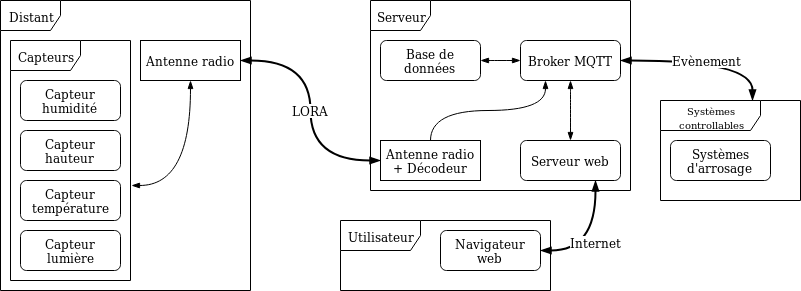
\includegraphics[scale=0.5]{graph.png}
	\end{centering}
	\caption{Infrastructure générale}
\end{figure}

\section{Résultats attendus}

Les résultats attendus sont une gestion intelligente et automatisée des ressources, la première étant l'eau.
Les interventions de l'utilisateur devront être minimes, tout en lui assurant des possiblités de contrôle et de surveillance des différents appareils de son exploitation.

\end{document}